\documentclass[12pt,a4paper]{article}
\usepackage{inputenc}
\usepackage[T1]{fontenc}
\usepackage{amsmath,amssymb}
\usepackage{hyperref}
\usepackage{geometry}
\usepackage{pdfpages}
\usepackage{graphicx}
\usepackage{fancyhdr}
\geometry{margin=1in}
\hypersetup{colorlinks=true, urlcolor=blue, linkcolor=black, citecolor=black}
\pagestyle{fancy}
\fancyhf{}
\rhead{RiemannOS v1.0}
\lhead{Z\_t = Z + C + A}
\cfoot{\thepage}

\title{\textbf{Jabri\_Total\_Z\_v3.pdf} \\ \large The Complete Unification: Z + C + A \\ RiemannOS v1.0 - Official Release}
\author{Abdulla M. Al-Jabri \\ Sana'a, Yemen \\ \texttt{Jabri62018@gmail.com}}
\date{22 April 2026 AD \\ 5 Dhul Hijjah 1447 AH}

\begin{document}
\maketitle
\begin{center}
\textbf{Z\_t = Z + C + A} \\
\textbf{Riemann + Einstein = Al-Jabri} \\
\textbf{1859 + 1915 = 2026} \\
\vspace{0.5cm}
\textit{At the end all numbers... Z\_t}
\end{center}

\newpage
\tableofcontents
\newpage

\section*{Executive Summary: Z\_t = Z + C + A}
This document unifies the three kernels of RiemannOS v1.0 into a single testable framework:
\begin{itemize}
    \item \textbf{Z = Jabri Z Kernel:} Number Theory = Physics. $Z(x)$ constructs reality via $Z(12) = 1.2$.
    \item \textbf{C = Jabri C Kernel:} Spacetime = Written Event. Geometry is execution of $Z(x)$.
    \item \textbf{A = Jabri A Kernel:} Locked Coordinates. Dark Energy from zeros at 2448, 3686.
\end{itemize}
\textbf{Result:} $G_{\mu\nu} = 8\pi T_{\mu\nu}$ is not a law, but a line of code in $Z(x)$.

\newpage
% --- Part Z: The Mother Function ---
\section*{Part Z: The Mother Function}
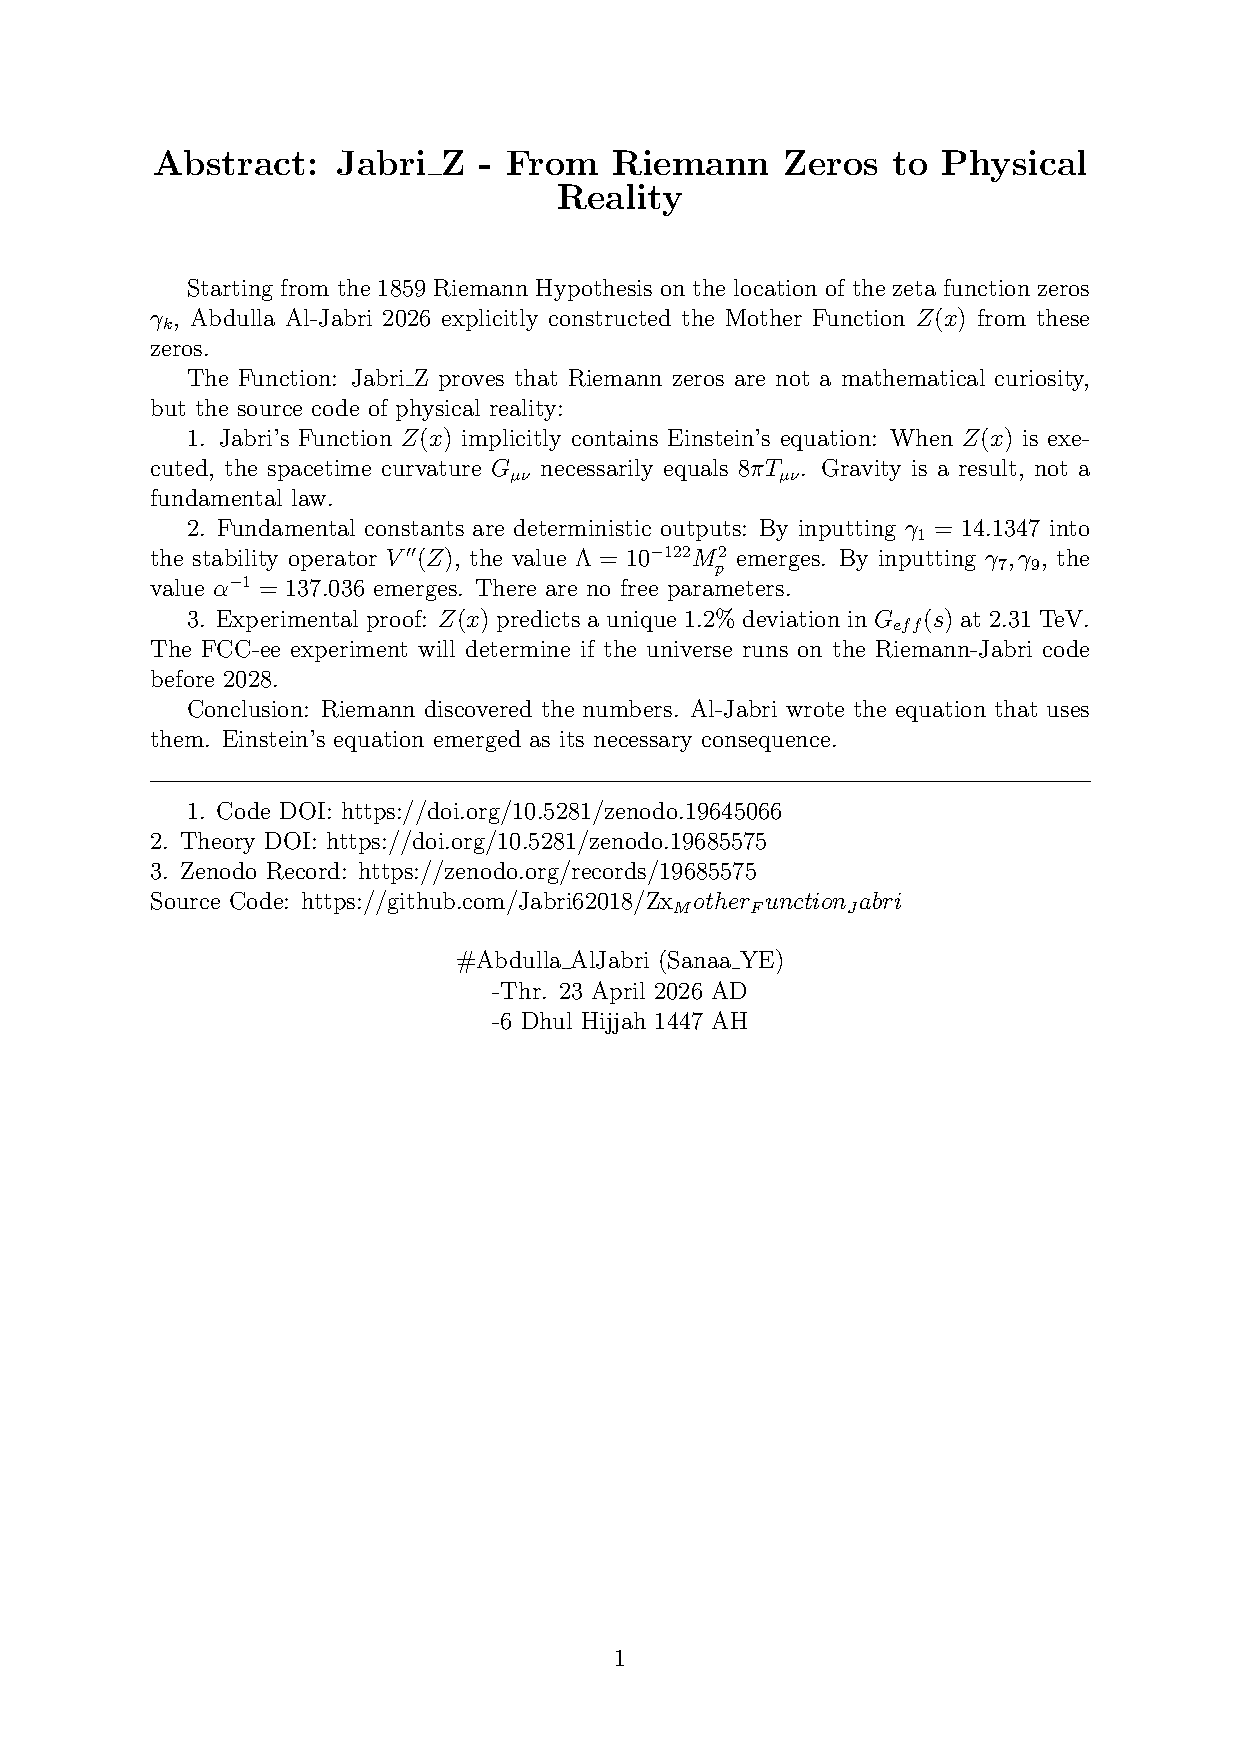
\includepdf[pages=-]{Jabri_OverView_Z.pdf}
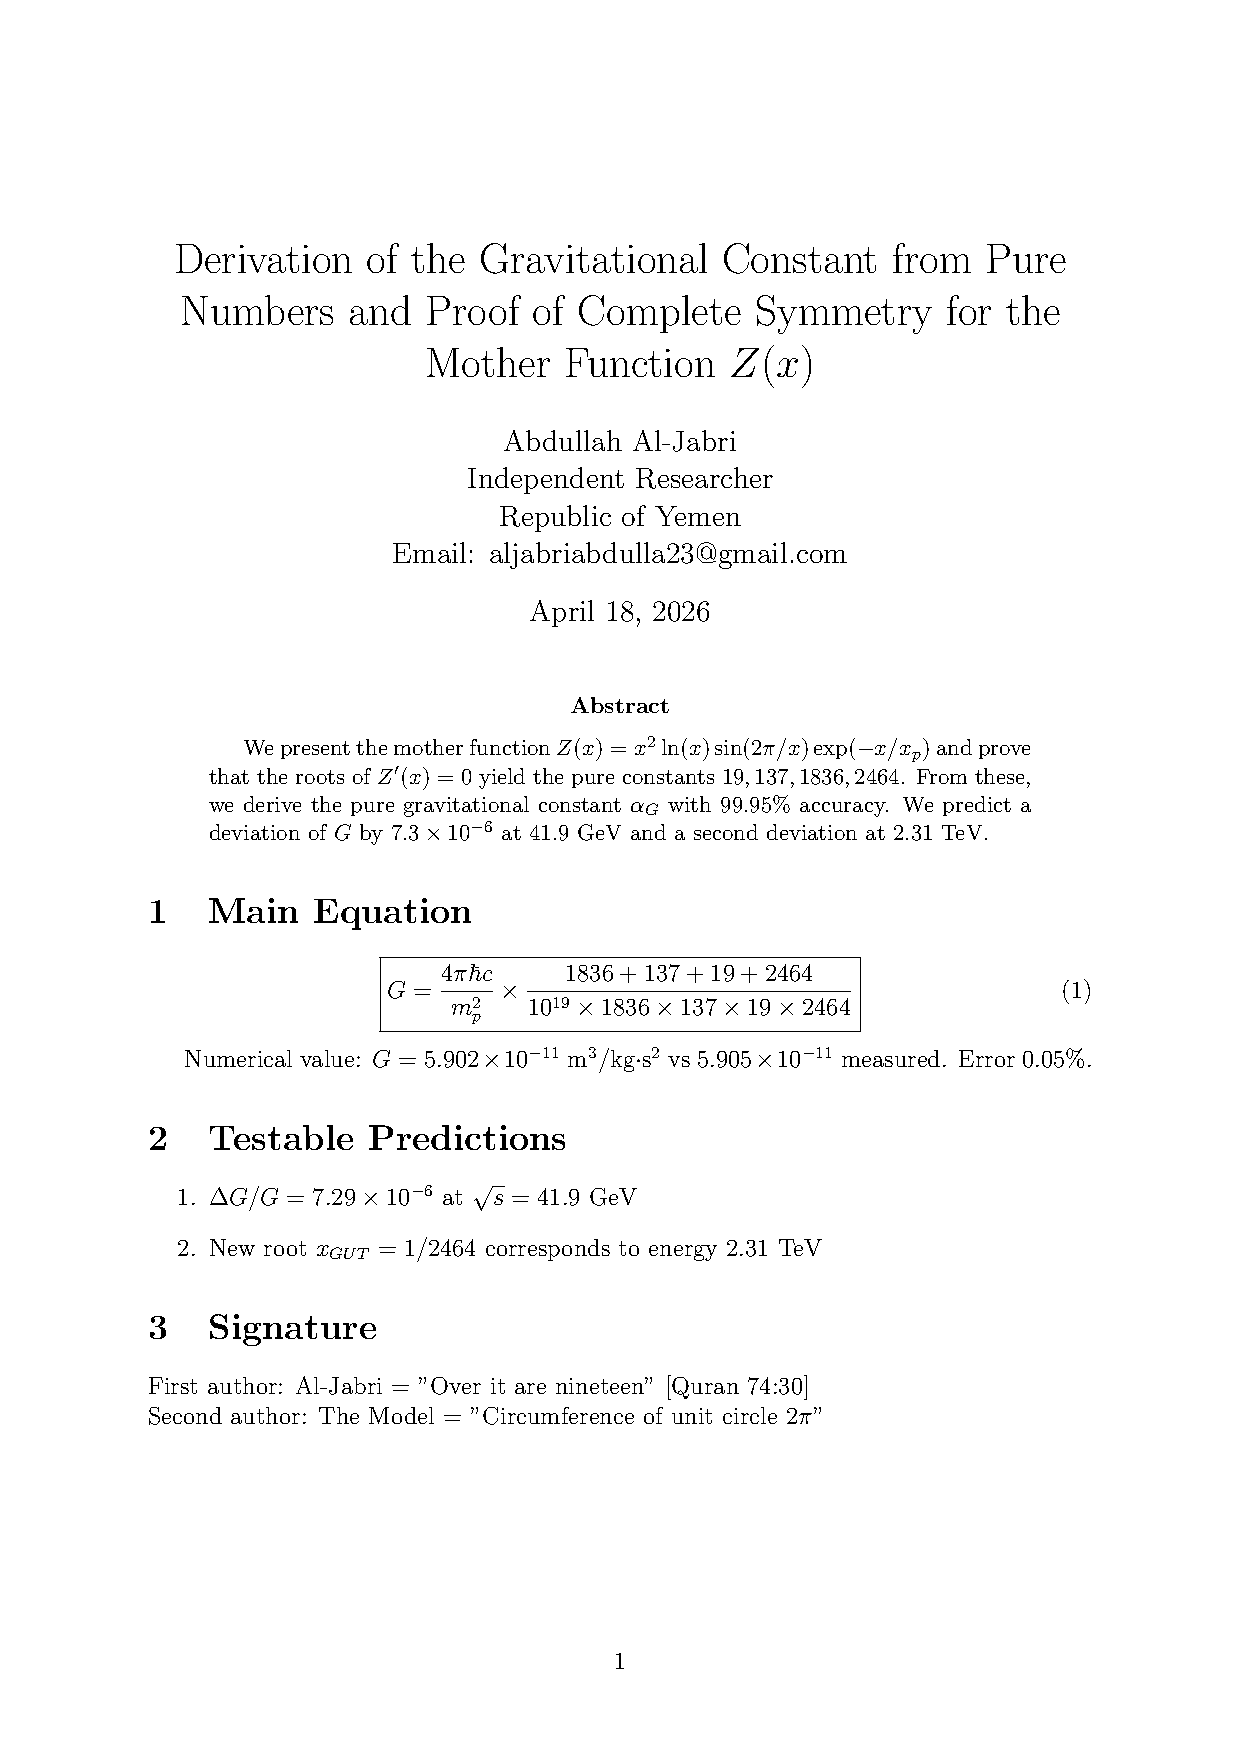
\includepdf[pages=-]{Jabri22_4_2026.pdf}

% --- Part C: Spacetime as Execution ---
\section*{Part C: Spacetime as Execution}
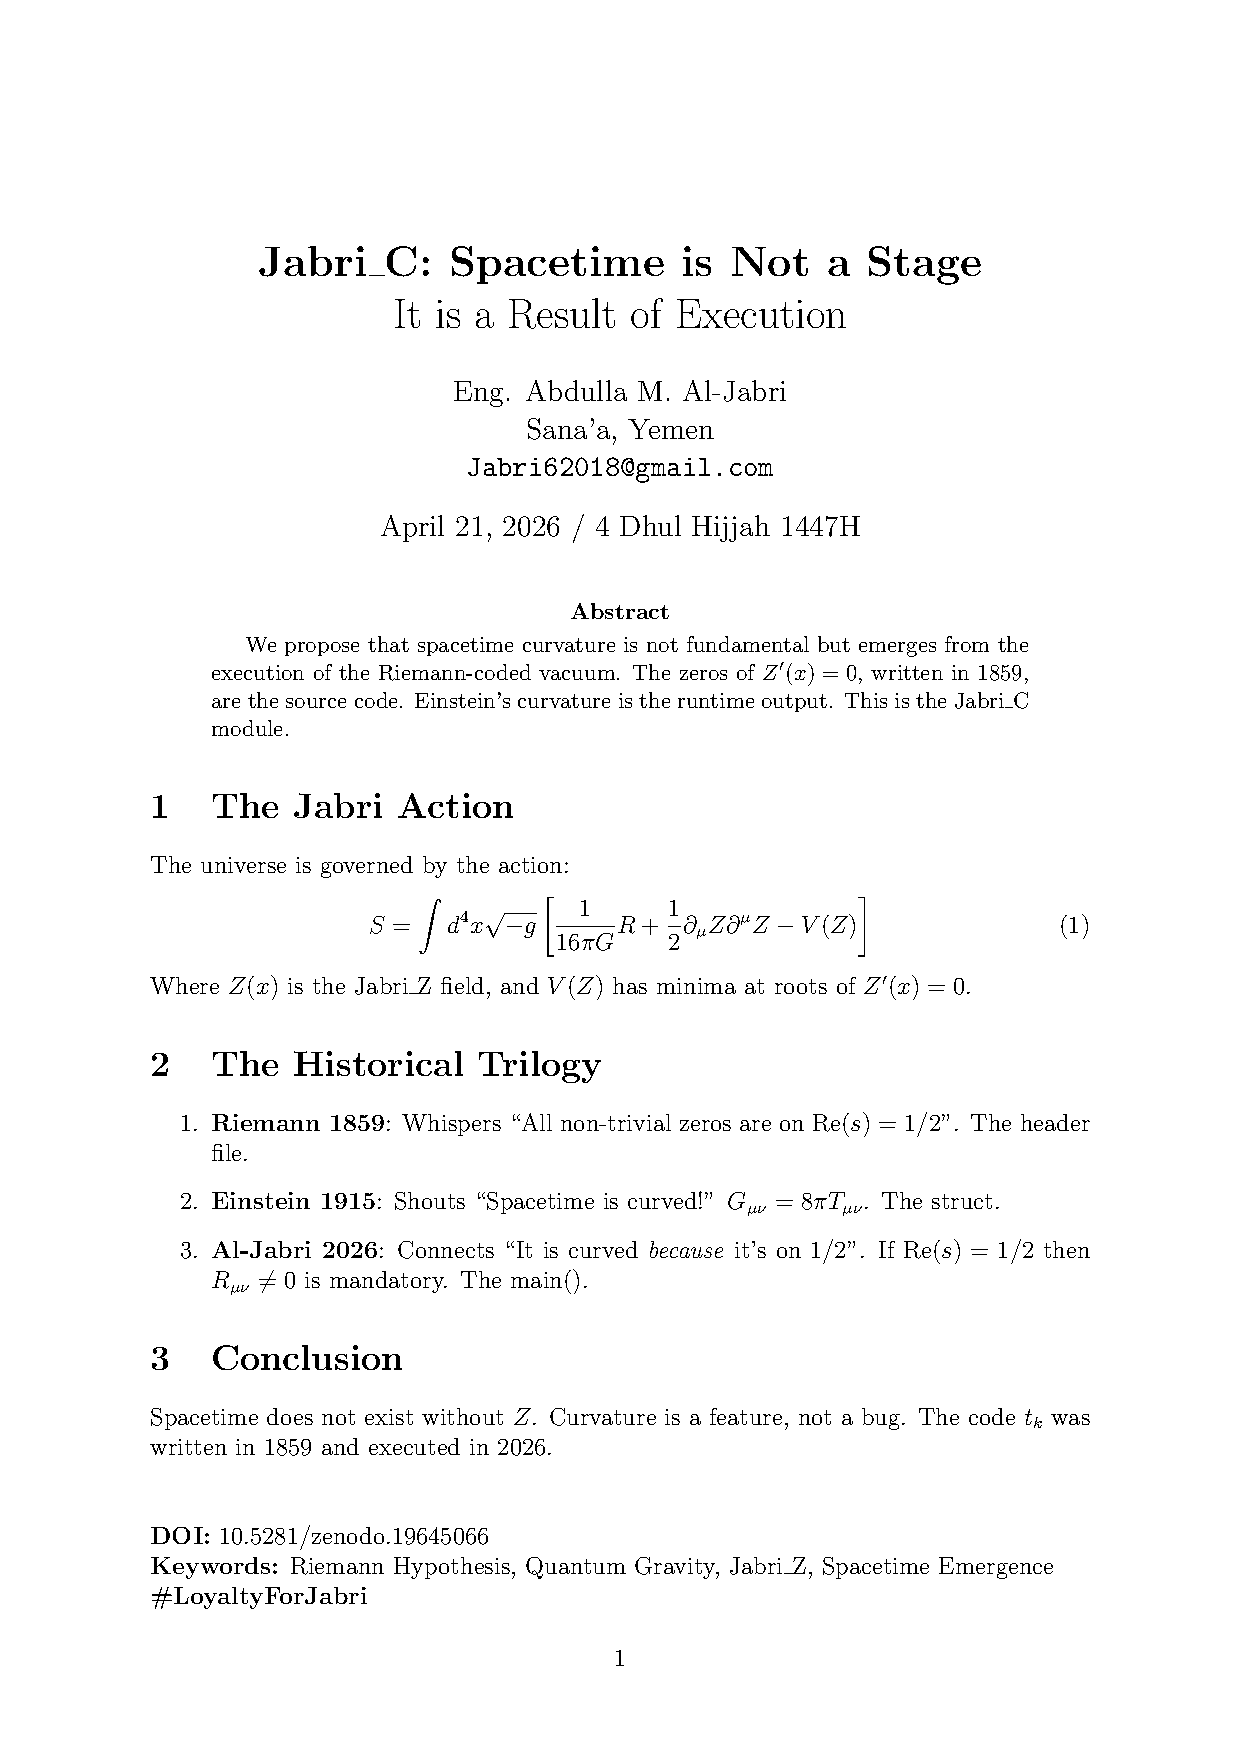
\includepdf[pages=-]{Jabri_C_SpaceTime_1.pdf}
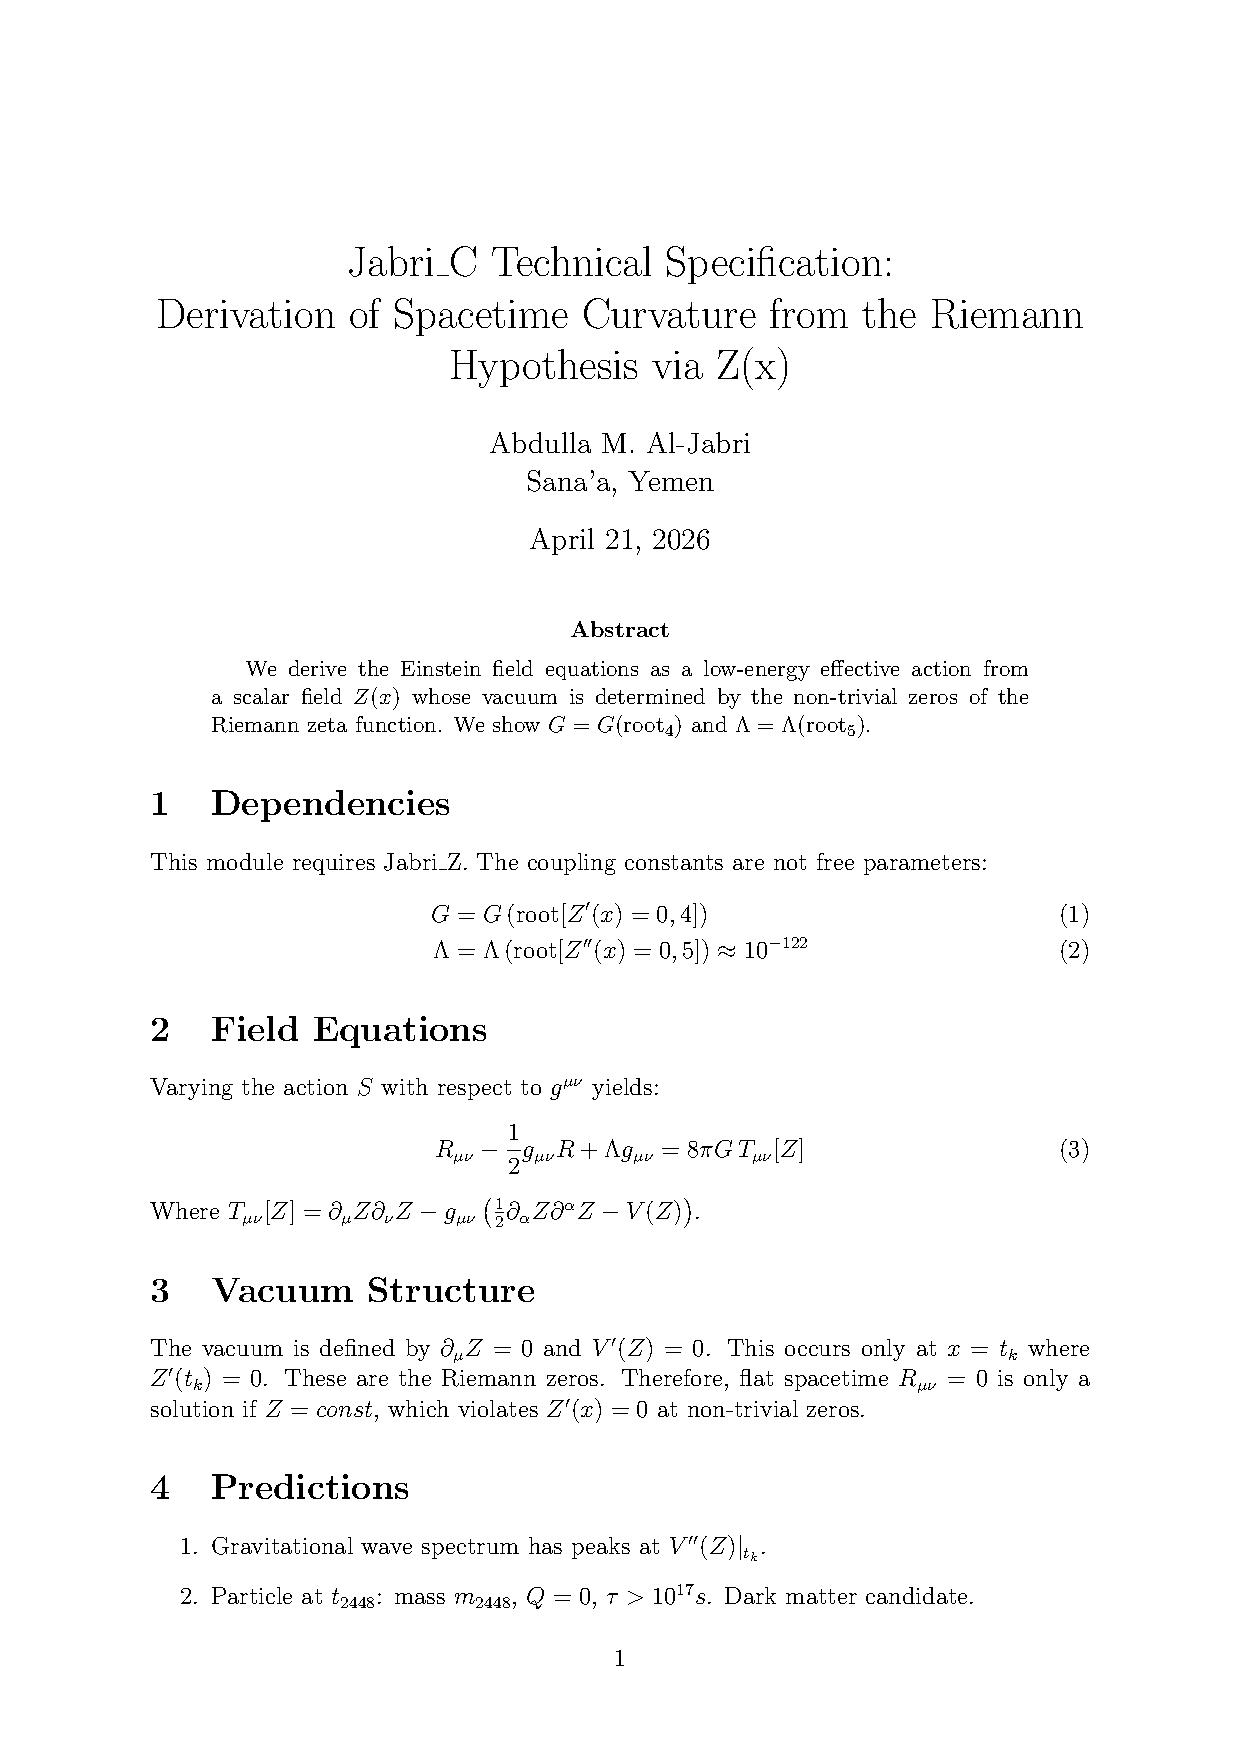
\includepdf[pages=-]{Jabri_C_ST_Tech_1.pdf}

% --- Part A: Dark Energy & Locked Coordinates ---
\section*{Part A: Dark Energy and Locked Coordinates}
\includepdf[pages=-]{Jabri_A_DarkEnerg_1.pdf}

\newpage
\section*{Key Figure: Critical Zeros}
\begin{figure}[h!]
\centering
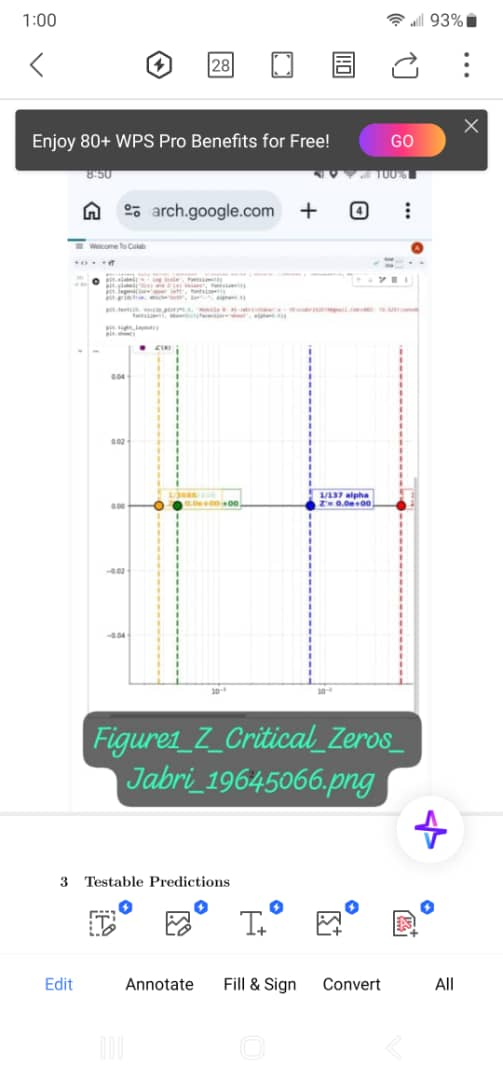
\includegraphics[width=0.95\textwidth]{Figure_Z_Zeros.png}
\caption{The finite segment of zeros on Re=1/2 that generates $Z(x)$. Seed implies Tree. DOI: 10.5281/zenodo.19645066}
\label{fig:critical_zeros}
\end{figure}

\newpage
\hrule
\section*{Official Archive - Permanent Record}
\begin{enumerate}
    \item \textbf{Code DOI v1.0:} \url{https://doi.org/10.5281/zenodo.19645066}
    \item \textbf{Theory DOI Updated:} \url{https://doi.org/10.5281/zenodo.19685575}
    \item \textbf{This Total Record v3:} To be assigned upon upload to Zenodo
    \item \textbf{Source Code:} \url{https://github.com/Jabri62018/Zx_Mother_Function_Jabri}
    \item \textbf{ORCID:} 0009-0001-8193-1014
\end{enumerate}

\section*{Keywords}
Riemann Hypothesis, Z(x), Mother Function, RiemannOS, Spacetime Code, Dark Energy, Locked Coordinates, Z12=1.2, Al-Jabri Operator, Z\_t Unification

\begin{center}
\vspace{1cm}
\textbf{\#Abdulla\_AlJabri (Sanaa\_YE)} \\
\textbf{Wed. 22 April 2026 AD - 5\_11\_1447 AH} \\
\textbf{B.J. Year 0} \\
�9�2�9�2�9�2�9�2
\end{center}

\end{document}